\section{Designing a test}
\paragraph{}
There are two ways to create a testing scene.
The original way is to write code for everything, including scene graph buildup.
The new way is to use the UI of \ER\ to create the scene graph,
and only write code to change the scene for each query.
In both cases, the code for interaction and logging has to be written.

But before code is written, the test has to be designed.
This is easiest in the steps seen in figure \ref{imgWorkflow}.


\subsection{Play Phase}
\paragraph{}
In this phase, the look of the test is created.
By placing objects in the scene, varying parameters and viewing it in 3D, it is easy to create a scene that will look good and can be seen easily in the test.

What kind of object to place is an important decision.
If binocular fusion has to be ensured, using random dot stereograms\ref{Stereogram} is a good choice.
Stereograms are created as textures on pixel planes, since they need to be reproduced pixel exact on screen.

Easy geometric shapes like parallelepipeds, parallelograms or circles can be made directly in \ER,
for more complicated shapes, meshes have to be made in a 3D modeling software.

Meta objects/container nodes play an important role in \ER's scene graph design.
Objects that need to be seen with a different camera than the scene are placed as sub-object of a camera node.
Similarly, lit objects are sub-objects of a light node, transformed objects are sub-objects of a transformation node and objects with non-standard depth ordering are sub-objects of a depth node.

\paragraph{Parameter Selection}
When deciding on the look of the scene, the position, size and other parameters are very important.
The limits of placement in depth and on screen need to be known. Objects that exceed those limits can not be perceived easily.
The points of interest should be limited in a test, more possible positions of the stimuli increase the difficulty in balancing.
Common points are the near- and far-points, as well as the zero parallax plane.

The object properties such as texture, size and orientation are also important.
It depends on the test what is optimal, but high contrast black and white textures make a good initial choice.


\subsection{Design Phase}

%\begin{figure*}[htb]
\begin{center}
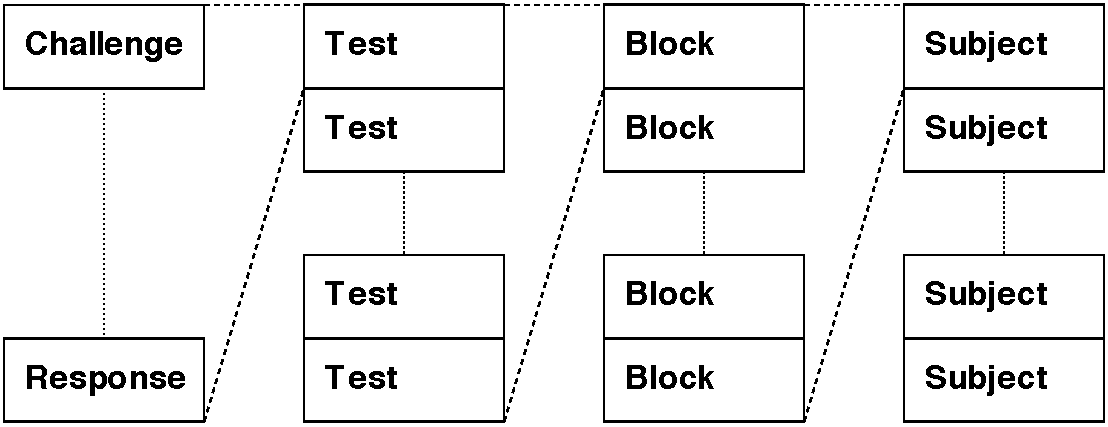
\includegraphics[width=7.25cm]{media/test.pdf}
%\caption{A diagram of a possible scene graph.\label{imgScene}}
\end{center}
%\end{figure*}

\paragraph{}
In the design phase, the decision what to test and how to test it is made.
Most psychological tests have to be designed in such a way, that the influence of factors outside the scope of the experiment can be compensated as much as possible.
Factors have to be counterbalanced to eliminate them,
or measured to account for them.
Every free variable, a factor that is not eliminated, requires additional samples to measure.

Knowledge in the domain of experimental psychology is of great value in this part of the test.

\paragraph{Test Sample}
A test sample is a single piece of data.
It is usually gathered by presenting a stimuli to the test subject,
and measuring the response, and the response time.
The parameters describing a stimuli and the response make up the data of the sample.
Some tests might not follow this pattern.

\paragraph{Blocks}
A block is a grouping of test samples.
The order of the test samples should be random within a block, but every block should be equivalent to all others.
The results gathered inside a block are only used together.
This allows the measurement of changes in the data gathered during a whole experiment by comparing results between blocks.

\paragraph{Subjects}
The selection of subjects is a factor that can not be neglected.
Are test subjects selected randomly from a big pool, or are they selected from volunteers,
is the age and physiological fitness a factor?
Under which conditions the subjects are rejected can influence the test design.

The difficulty of the test might make it not solvable by everyone.
The right test has to be chosen for the right target subject group.
Different tests are not neccessarily comparable.


\subsection{Implement}
\paragraph{}
Implementing the test involves creating a lua file containing scene graph description,
scene mechanic description as lua code and the creation of media files.
Scenes can be creates either in pure lua, or with the help of the \ER\ user interface.

\subsubsection{Pure Lua}
\paragraph{}
Pure lua tests can be structured without any additional restrictions.
It is however advised to follow some guidelines to make the code easier readable
and maintainable.

Important parameters, especially those that are used in several places, should be stored in variables.
Everything relevant should be commented.

The next thing to do in a pure lua scene is to set up the scene graph.
All objects should be created and added to the scene graph.
Make sure to keep pointers to those objects you want to change later.
Next, the data structures for the test is set up.
Tables of possible positions that can be randomly permuted have shown to be useful.
It would also be possible to dynamically generate new positions, depending on the design of the test.

\paragraph{Interaction}
The scene interaction is done in event handlers.
Usually, the \texttt{keyDown} or \texttt{keyUp} handler is registered to handle user input.
The handler method checks if the user input is correct, logging the result of the check.
Then it changes the scene graph to represent the next stimulus, usually by moving objects, or changing their texture or other parameters.
The next stimulus is written to the log to start the timer for the next test.

The \texttt{update} handler can be used to animate the scene,
or to do other time based activities, such as waiting.


\subsubsection{UI assisted}
\paragraph{}
At the heart, ui assisted test creation is similar to the pure lua method.
The only difference is that the scene graph is created in the user interface.
During the design and play phase, such a scene graph is usually already created and can be reused.

The interaction is defined exactly as in the pure lua method.
An additional code file can be added in the user interface, and should be used to store the code.
Files managed by the user interface get rewritten every time they are saved, overwriting any custom code they contain.


\subsection{Log Format}
\paragraph{}
What to log and how to log it is decided by the scene design.
In most tests it is advised to log all changing parameters, as well as all user input.
The common form of query-response test has at least one special log entry that identifies the start of a new query, and one that identifies it's end.
The time stamps of those events are used to calculate response time.


